\begin{figure}[bth!]
	\begin{center}
	   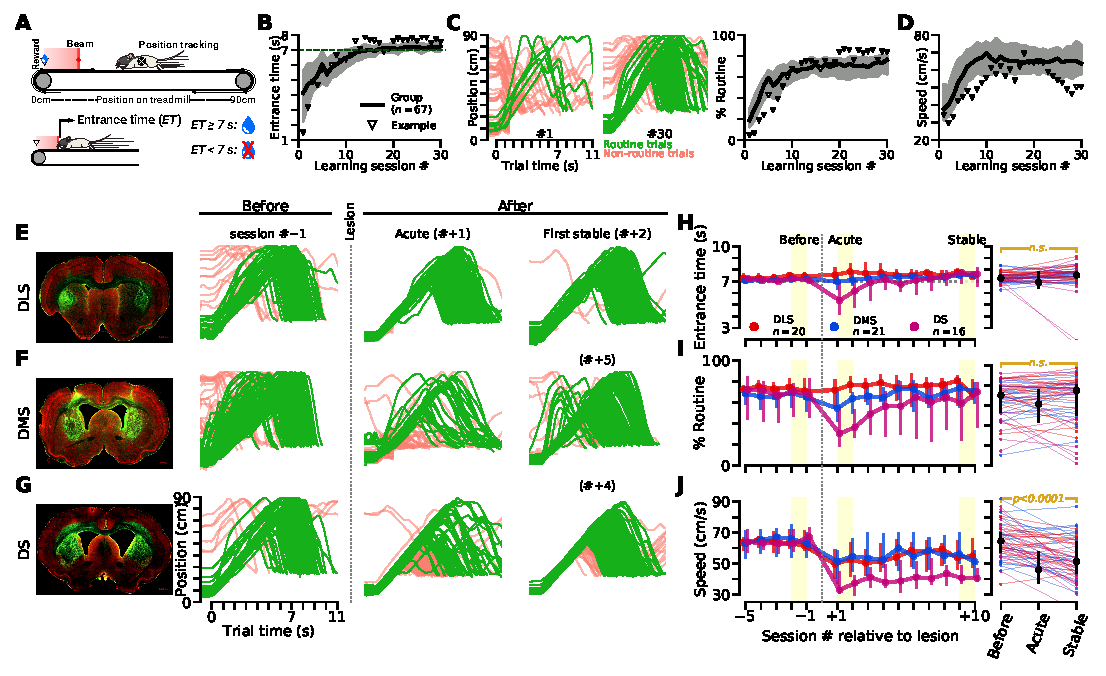
\includegraphics[width=\textwidth]{ch-lesion/figures/Task_Example_Group.pdf}
	   \caption
	   {\textbf{The dorsal striatum is necessary to invigorate the running component of a motor routine.}
	   \textbf{(A)} Experimental apparatus and task rules.
	   \textbf{(B)} Entrance time across training sessions for all the rats trained in this task.  
   Shaded area represents the interquartile range.
   \textbf{(C)} Trajectories of an example animal on the treadmill, for all the trials performed during sessions \#1 and \#30 (left).
   Percentage of trials during which animals performed the wait-and-run routine, across sessions (right).
   \textbf{(D)} Running speed when animals ran toward the reward area, across sessions.
   Triangles in B to D indicate the changes in performance for the example animal whose trajectories are shown in C (left).
	   \textbf{(E-G)} Histology ($1^{st}$ column, GFAP in green shows gliosis, red is NeuN) and trajectories of single animals with bilateral lesions of the dorsolateral, dorsomedial and dorsal striatum (E: DLS, F: DMS: G: DS).
	   \# indicates session number relative to lesion break.
	   \textbf{(H-J)} Left, Time course of the lesion effect on ET (H), percentage of routine usage (I) and running speed (I).
	   Right, group data statistical comparison before vs after lesion (10,000 resamples).
	   Trajectories in C, E, F and G are cut after ET.
	   }
	   \label{fig:lesion:task}
	\end{center}
   \end{figure}